\chapter{Random Forests}
\label{chap:randomforest}

\begin{myremark}[Algorithmusart in diesem Kapitel]
Funktionsart: \textbf{Klassifikation}. \\
Umsetzungsart: \textbf{selbstlernend} (Ensembleverfahren).
\end{myremark}

\begin{myremark}
Der \textbf{Random Forest} baut auf dem Entscheidungsbaum auf (Kapitel~\cref{chap:entscheidungsbaum}) und macht ihn
durch \enquote{Ensembling} deutlich robuster. Diese Methode setzt Kenntnisse aus Kapitel~\cref{chap:entscheidungsbaum} voraus.
\end{myremark}

\section{Grundidee: Viele Bäume, eine Entscheidung}

\begin{mydefinition}[Random Forests]
Ein \textbf{Random Forest} kombiniert viele \textbf{zufällig variierte} Entscheidungsbäume.
Die finale Klassifikation entsteht durch \textbf{Mehrheitsabstimmung} aller Bäume.
\end{mydefinition}

Durch zwei Mechanismen wird jeder Baum bewusst \enquote{anders} gemacht:
\begin{enumerate}
    \item \textbf{Bagging:} Jeder Baum trainiert auf einer zufälligen Stichprobe der Daten
          (mit Zurücklegen).
    \item \textbf{Feature-Subsampling:} An jedem Knoten wird nur eine zufällige Teilmenge
          der Merkmale betrachtet.
\end{enumerate}

\begin{figure}[H]
    \centering
    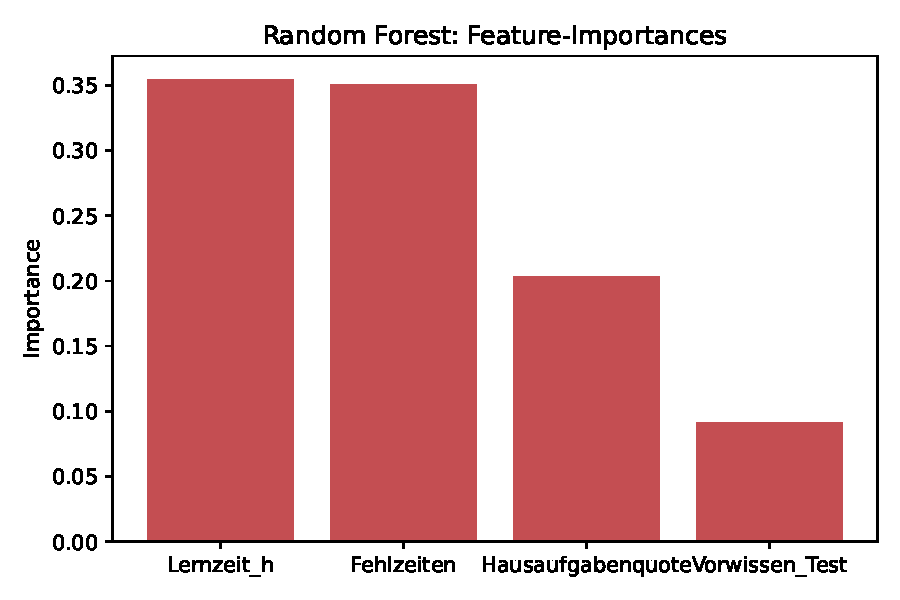
\includegraphics[width=0.72\textwidth]{Grundlagen_Info/10_KI_und_Algorithmen/Figures/random_forest_feature_importance.pdf}
    \caption{Feature-Importances eines Random-Forest-Modells}
    \label{fig:rf-importance-15}
\end{figure}

\section{Feature Importance}

\begin{mydefinition}[Feature Importance]
Der Random Forest kann angeben, wie stark jedes Merkmal zur Entscheidung beiträgt.
Ein Merkmal ist wichtig, wenn Splits auf ihm die Unreinheit (Gini) stark reduzieren.
\end{mydefinition}

\begin{myexercise}[Vergleich: Baum vs.\ Wald]
Diskutieren Sie in Zweiergruppen:
\begin{itemize}
    \item Warum kann ein einzelner Baum schnell \enquote{auswendig lernen}?
    \item Warum ist ein Wald oft robuster gegen Overfitting?
    \item Welche Nachteile hat der Random Forest gegenüber einem einzelnen Baum?
\end{itemize}
\end{myexercise}

\section{Hyperparameter}

\begin{mychallenge}[Hyperparameter verstehen und tunen]
Recherchieren und erklären Sie kurz:
\begin{itemize}
    \item \texttt{n\_estimators} -- Anzahl Bäume
    \item \texttt{max\_depth} -- maximale Tiefe je Baum
    \item \texttt{min\_samples\_leaf} -- Mindestgrösse eines Blatts
\end{itemize}
Testen Sie im Notebook verschiedene Werte und dokumentieren Sie den Effekt
auf Trainings- und Testgenauigkeit.
\end{mychallenge}

\section{Gesellschaftliche Aspekte: Black-Box-Problem und Bias-Verstärkung}

\begin{mydefinition}[Ensemble-Risiken]
Obwohl Random Forests durch Ensembling robuster werden, entsteht gleichzeitig ein \enquote{Black-Box}-Problem: Man kann nicht mehr nachvollziehen, warum eine konkrete Entscheidung getroffen wurde. Feature Importance gibt nur einen aggregierten Überblick, sagt aber nichts über einzelne Vorhersagen aus.
\end{mydefinition}

\begin{myexample}[Hiring-System mit Random Forest]
Ein Unternehmen trainiert einen Random Forest auf 10 Jahren historischer Einstellungsdaten. Das Modell hat 99\% Accuracy auf den Testdaten und wird deployed. Feature Importance zeigt: \enquote{Berufserfahrung} und \enquote{Universität} sind am wichtigsten. Ein Kandidat wird abgelehnt. Das System kann nicht erklären, warum -- es ist eine Kombination von hunderten versteckten Regeln über hunderten Bäumen.

\textbf{Problem:} Wenn die Trainingsdaten systematisch diskriminierend waren (z.~B. Frauen wurden weniger häufig eingestellt), lernt das Random Forest diese Verzerrung und verstärkt sie durch Skalierung und Black-Box-Natur.

\textbf{Real-World-Link:} \href{https://www.reuters.com/article/world/insight-amazon-scraps-secret-ai-recruiting-tool-that-showed-bias-against-women-idUSKCN1MK0AG/}{Amazon stoppt KI-Hiring-System wegen Geschlechtsdiskriminierung (2018)}
\end{myexample}

\begin{mychallenge}[Interpretierbarkeit vs. Genauigkeit]
Viele Unternehmen wählen Random Forests, weil sie genauer sind als Entscheidungsbäume. Diskutieren Sie:
\begin{enumerate}
    \item Warum ist Interpretierbarkeit in Hochrisiko-Entscheidungen (Kredite, Hiring, medizinische Diagnose) wichtiger als maximale Accuracy?
    \item Wie würde man einen Random Forest in einem Hiring-System überprüfen, um sicherzustellen, dass er nicht diskriminiert?
    \item Welche Rolle spielen externe Audits und Regulierung?
\end{enumerate}
\begin{myanswer}
    \begin{enumerate}
        \item Betroffene Personen haben ein Recht zu verstehen, warum Entscheidungen gegen sie getroffen wurden. Accuracy allein legitimiert keine Diskriminierung.
        \item Demografische Parity-Tests, Analyse der Fehlerquoten über Gruppen hinweg, explizite Fairness-Metriken, externe Audits.
        \item Regulierung (z.~B. EU-AI-Act) erzwingt Transparenz und Audit für High-Risk-Systeme, da Marktanreize allein oft nicht ausreichen.
    \end{enumerate}
\end{myanswer}
\end{mychallenge}

\begin{myremark}[Notebook]
Praktische Umsetzung inkl. Übungen:
\href{\notebookbaseurl02_Random_Forest_Classification.ipynb}{\texttt{02\_Random\_Forest.ipynb}}
\end{myremark}
